%%%%%%%%%%%%%%%%%%%%%%%%%%%%%%%%%%%%%%%%%%%%%%%%%%%%%%%%%%%%%%%%%%%%%%%%%%%
% Machine Learning Basics %
%%%%%%%%%%%%%%%%%%%%%%%%%%%%%%%%%%%%%%%%%%%%%%%%%%%%%%%%%%%%%%%%%%%%%%%%%%%
\section{Structuring Data without Neural Networks}
\label{sec:structuring_data}
Deep learning with neural networks is very much at the forefront of the recent renaissance in machine learning. However,
machine learning is not synonymous with neural networks.
There is a wealth of machine learning approaches without neural networks, and the boundary between them and conventional statistical analysis is not always sharp.

It is a common misconception that neural network techniques would always outperform these approaches. In fact, in some cases, a simple linear method could achieve faster and better results. Even when we might eventually want to use a deep network, simpler approaches may help to understand the problem we are facing and the specificity of the data so as to better formulate our machine learning strategy. In this chapter, we shall explore machine learning approaches without the use of neural networks. This will further allow us to introduce basic concepts and the general form of a machine learning workflow.

\subsection{Principle component analysis}

At the heart of any machine learning task is data. In order to choose the most appropriate machine learning strategy, it is essential that we understand the data we are working with. However, very often, we are presented with a dataset containing many types of information, called \emph{features}\index{features} of the data. Such a dataset is also described as being high-dimensional. Techniques that extract information from such a dataset are broadly summarised as \emph{high-dimensional inference}.
For instance, we could be interested in predicting the progress of diabetes in patients given features such as age, sex, body mass index, or average blood pressure. Extremely high-dimensional data can occur in biology, where we might want to compare gene expression pattern in cells.
Given a multitude of features, it is neither easy to visualise the data nor pick out the most relevant information. This is where \textit{principle component analysis} (PCA) can be helpful.

Very briefly, PCA is a systematic way to find out which feature or combination of features varies the most across the data samples. We can think of PCA as approximating the data with a high-dimensional ellipsoid, where the principal axes of this ellipsoid correspond to the principal components. A feature, which is almost constant across the samples, in other words has a very short principal axis, might not be very useful. PCA then has two main applications: (1) It helps to visualise the data in a low dimensional space and (2) it can reduce the dimensionality of the input data to an amount that a more complex algorithm can handle.
\vspace{12pt}

\noindent
\textbf{PCA algorithm}\vspace{3pt}\\
Given a dataset of $m$ samples with $n$ data features, we can arrange our data in the form of a $m$ by $n$ matrix $X$ where the element $x_{ij}$ corresponds to the value of the $j$th data feature of the $i$th sample. We will also use the \emph{feature vector} $\bm{x}_i$ for all the $n$ features of one sample $i=1,\ldots,m$. The vector $\bm{x}_i$ can take values in the \emph{feature space}, for example $\bm{x}_i \in \mathbb{R}^n$. Going back to our diabetes example, we might have $10$ data features. Furthermore if we are given information regarding $100$ patients, our data matrix $X$ would have $100$ rows and $10$ columns.

The procedure to perform PCA can then be described as follows:

\begin{algbox}[Principle Component Analysis]{alg:pca}
\begin{enumerate}
    \item 
    Center the data by subtracting from each column the mean of that column,
    \begin{equation}
        \bm{x}_i \mapsto \bm{x}_{i} - \frac{1}{m} \sum_{i=1}^{m} \bm{x}_{i}.
      %  x_{ij} \longrightarrow x_{ij} - \frac{1}{m} \sum_{i=1}^{m} x_{ij}.
    \end{equation}
    This ensures that the mean of each data feature is zero.
    \item 
    Form the $n$ by $n$ (unnormalised) covariance matrix
    \begin{equation}
        C = {X}^{T}{X} = \sum_{i=1}^{m} \bm{x}_{i}\bm{x}_{i}^{T}.
        \label{eqn: PCA Covariance Matrix}
    \end{equation} 
    \item 
    Diagonalize the matrix to the form $C = {X}^{T}{X} = W\Lambda W^{T}$, where the columns of $W$ are the normalised eigenvectors, or principal components, and $\Lambda$ is a diagonal matrix containing the eigenvalues. It will be helpful to arrange the eigenvalues from largest to smallest.
    \item 
    Pick the $l$ largest eigenvalues $\lambda_1, \dots \lambda_l$, $l\leq n$ and their corresponding eigenvectors $\bm{v}_1 \dots \bm{v}_l$. Construct the $n$ by $l$ matrix $\widetilde{W} = [\bm{v}_1 \dots \bm{v}_l]$.
    \item 
    Dimensional reduction: Transform the data matrix as
    \begin{equation} \label{eqn: PCA Dimensional Reduction}
        \widetilde{X} = X\widetilde{W}.
    \end{equation} 
    The transformed data matrix $\widetilde{X}$ now has dimensions $m$ by $l$.
\end{enumerate}
\end{algbox}

We have thus reduced the dimensionality of the data from $n$ to $l$. Notice that there are actually two things happening: First, of course, we now only have $l$ data features. But second, the $l$ data features are new features and not simply a selection of the original data. Rather, they are a linear combination of them. Using our diabetes example again, one of the ``new'' data features could be the sum of the average blood pressure and the body mass index. These new features are automatically extracted by the algorithm.

But why did we have to go through such an elaborate procedure to do this instead of simply removing a couple of features? The reason is that we want to maximize the \textit{variance} in our data. We will give a precise definition of the variance later in the chapter, but briefly the variance just means the spread of the data. Using PCA, we have essentially obtained $l$ ``new'' features which maximise the spread of the data when plotted as a function of this feature. We illustrate this with an example.
\vspace{12pt}

\noindent
\textbf{Example}\vspace{3pt}\\
Let us consider a very simple dataset with just $2$ data features. We have data, from the Iris dataset~\footnote{\href{https://archive.ics.uci.edu/ml/datasets/iris}{https://archive.ics.uci.edu/ml/datasets/iris}}, a well known dataset on 3 different species of flowers. We are given information about the petal length and petal width. Since there are just $2$ features, it is easy to visualise the data. In Fig.~\ref{fig: Iris PCA}, we show how the data is transformed under the PCA algorithm.

\begin{figure*}[t]
  \centering
    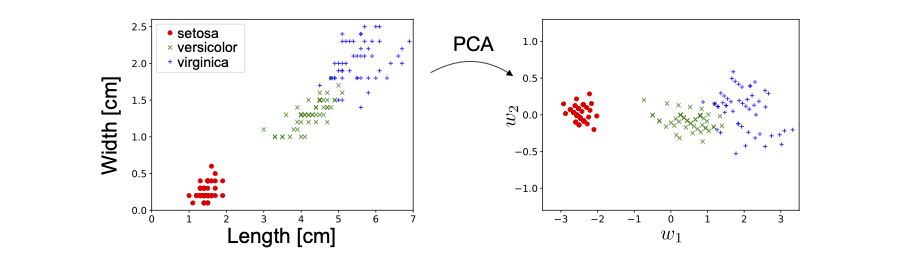
\includegraphics{Iris-PCA}
    \caption{\textbf{PCA on Iris Dataset.}}
\label{fig: Iris PCA}
\end{figure*}

%    \caption{HKA am Beispiel der Länge und Breite von Schwertlilien-Blütenblättern der drei Arten Borsten-Schwertlilien (iris setosa), verschiedenfarbige Schwertlilien (iris versicolor) und iris virginica.}

Notice that there is no dimensional reduction here since $l = n$. In this case, the PCA algorithm amounts simply to a rotation of the original data. However, it still produces $2$ new features which are orthogonal linear combinations of the original features:  petal length and petal width, i.e.
\begin{equation}
    \begin{split}
        w_1 &= 0.922 \times \textrm{Petal Length} + 0.388 \times \textrm{Petal Width}, \\
        w_2 &= -0.388 \times \textrm{Petal Length} + 0.922 \times \textrm{Petal Width}.
    \end{split}
\end{equation}
We see very clearly that the first new feature $w_1$ has a much larger variance than the second feature $w_2$. In fact, if we are interested in distinguishing the three different species of flowers, as in a classification task, its almost sufficient to use only the data feature with the largest variance, $w_1$. This is the essence of (PCA) dimensional reduction.

Finally, it is important to note that it is not always true that the feature with the largest variance is the most relevant for the task and it is possible to construct counter examples where the feature with the least variance contains all the useful information. However, PCA is often a good guiding principle and can yield interesting insights in the data. Most importantly, it is also \emph{interpretable}\index{interpretability}, i.e., not only does it separate the data, but we also learn \emph{which} linear combination of features can achieve this. We will see that for many neural network algorithms, in contrast, a lack of interpretability is a big issue.
